\documentclass[a4paper]{article}
\usepackage[T2A,T1]{fontenc}
\usepackage[utf8]{inputenc}
\usepackage[english, russian]{babel}
\usepackage{graphicx}
\usepackage[hcentering, bindingoffset = 10mm, right = 15 mm, left = 15 mm, top=20mm, bottom = 20 mm]{geometry}
\usepackage{multirow}
\usepackage{lipsum}
\usepackage{amsmath, amstext}
\usepackage{siunitx}
\usepackage{subcaption}
\usepackage{wrapfig}
\usepackage{adjustbox}
\usepackage{enumerate, indentfirst, float}
\usepackage{capt-of, svg}
\usepackage{icomma}

\usepackage[T2A]{fontenc} %кодировка
\usepackage[utf8]{inputenc} %кодировка исходного кода
\usepackage[english,russian]{babel} %локализация и переносы


\newenvironment{bottompar}{\par\vspace*{\fill}}{\clearpage}
 
\begin{document}


\begin{titlepage}
	\centering
	\vspace{5cm}
	{\scshape\LARGE МОСКОВСКИЙ ФИЗИКО-ТЕХНИЧЕСКИЙ ИНСТИТУТ (НАЦИОНАЛЬНЫЙ ИССЛЕДОВАТЕЛЬСКИЙ УНИВЕРСИТЕТ)
 \par}
	\vspace{4cm}
	{\scshape\Large Лабораторная работа №1 \par}
	\vspace{1cm}
	{\huge\bfseries Измерение температуры пламени  \par}
    {\huge\bfseries  методом обращения спектральных линий  \par}
\vspace{1cm}
\begin {figure}[H]
\begin{center}

\includegraphics[width=0.6\textwidth]{faki.png}
\end{center}
\end {figure}
\vspace{1cm}
\begin{flushright}
	{\large выполнили студенты 2 курса группы Б03-104}\par
	\vspace{0.3cm}
	{\LARGE Платонов Никита}\par
    \vspace{0.3cm}
    {\LARGE Алаторцев Кирилл}\par
    \vspace{0.3cm}
    {\LARGE Недопекин Валерий}\par
\end{flushright}
	\vfill
% Bottom of the page
	г. Долгопрудный, 2023 г.
\end{titlepage}


\section*{Аннотация:}

В данной работе мы исследуем переход ламинарного течения в пограничном слое к турбулентному. Жидкость в работе считаем несжимаемой. Справделивость применения теории несижмаемой жидкости приведена в \textbf{Приложении}. Далее мы определяем границу перехода между данными режимами, вычисляем критическое число Рейнольдса, при котором это происходит. После этого сравниваем его с полученным критическим числом Рейнольдса для ламинарного течения и для турбулентного. Ожидаем увидеть, что данная для турбулентного режима число Рейнольдса окажется больше, а для ламинарного - меньше, чем критическое число Рейнольдса перехода потока от ламинарного к турбулентному.




\section*{Цель работы:} 
Исследовать переход от ламинарного пограничного слоя к турбулентному, определить пограничный слов и критическое число Рейнольдса $Re_{\text{кр}}$ перехода.




\vspace{4cm}

\begin {figure}[H]
\begin{center}
\large{ВСЕ КОДЫ К РАБОТЕ МОЖНО НАЙТИ ЗДЕСЬ:}
\par

\includegraphics[width=0.3\textwidth]{qr.png}
\end{center}
\end {figure}




\newpage
\section*{Теоритические сведения:}
Процесс перехода течения в пограничном слое от ламинарного режима к турбулентному при малой интенсивности внешних возмущений состоит из трех условно разделяемых этапов: 

\begin{enumerate} 
  \item генерации волн в пограничном слое,
  \item  их усиления по законам линейной теории
  \item нелинейного разрушения ламинарного режима течения, когда возникают различные сложные явления, такие как взаимодействие возмущений, искажение среднего потока, вторичные течения, турбулентные пятна и т.п., которыми сопровождается окончательный переход к
турбулентности
\end{enumerate}
\par
Описанная последовательность стадий перехода схематически показана на 1.

\begin {figure}[H]
\begin{center}
\par
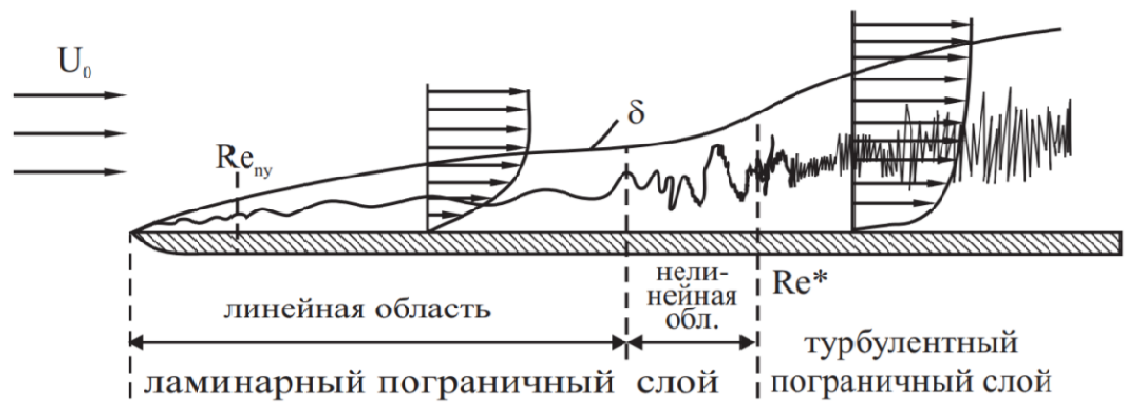
\includegraphics[width=0.9\textwidth]{01.png}
\caption{Стадии перехода в пограничном слое от ламинарного режима к турбулентному.}
\end{center}
\end {figure}

\subsection*{Описание первого эксперимента:}
Для определения числа Рейнольдса в первом эксперименте будем посредством изменения напряжения на
устройстве подачи воздуха менять скорость ядра; по полученным данным определим зависимость $u$/$u_\text{я}(Re)$, имеющую вид, показанный на рис. 2 слева. При ламинарном режиме течения в пограничном слое перед трубкой
полного напора увеличение скорости приведет к уменьшению толщины пограничного слоя и увеличению отношения $u$/$u_\text{я}$ . Когда переход будет происходить непосредственно перед трубкой полного напора, увеличение
скорости приведет к тому, что трубка будет все глубже погружаться в быстро нарастающий по координате $x$ турбулентный пограничный слой (2, слева), а это, в свою очередь приведет к уменьшению $u$/$u_\text{я}$.

\begin {figure}[H]
\begin{center}
\par
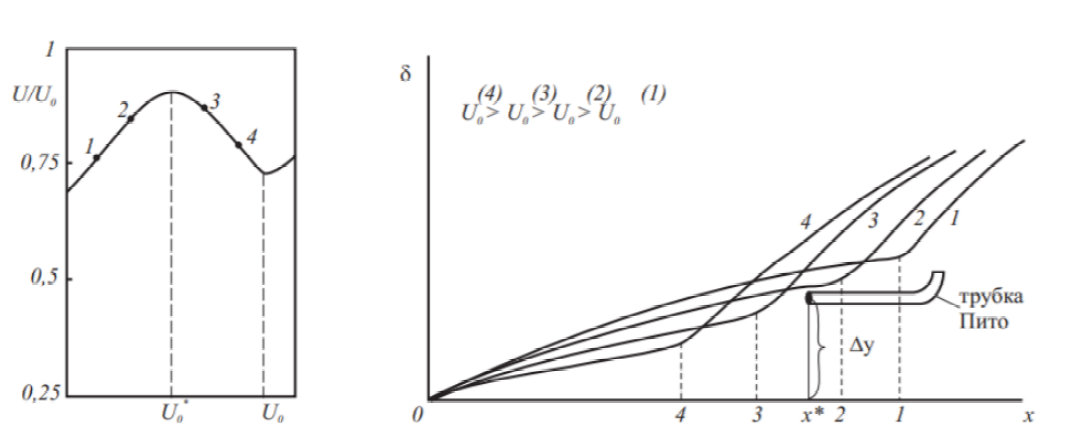
\includegraphics[width=0.9\textwidth]{02.png}
\caption{ К определению числа Рейнольдса перехода к турбулентности в пограничном слое при $x* = const$ и $U_0 = var$.}
\end{center}
\end {figure}

Тогда максимум зависимости $u$/$u_\text{я}$ от $Re$ будет соответствовать смене режима течения в пограничном слое
в месте, где будет установлена трубка полного напора.


\subsection*{Описание второго эксперимента:}
Во втором эксперименте будем проводить при двух определённых скоростях ядра потока (соответствующих ламинарному и турбулентному режимам), перемещая трубку Пито от стенки трубы к её центру. В результате
получим профили скоростей в ламинарином и турбулентном режиме (похоже на 3, изображающий поведение
профиля скоростей на пластине).

\begin {figure}[H]
\begin{center}
\par
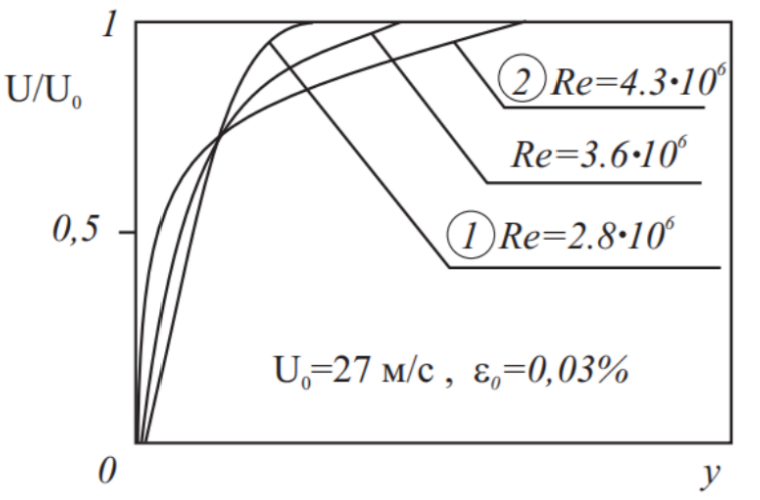
\includegraphics[width=0.5\textwidth]{03.png}
\caption{ Профили скорости в пограничном слое на пластине при переходе к турбулентности: 1 – ламинарное
течение, профиль Блаузиуса; 2 – турбулентное течение, закон степени 1/7, $\delta$ = 17 мм.}
\end{center}
\end {figure}



\subsection*{Рассчетные формулы:}
В реальных жидкостях и газах всегда имеет место прилипание к стенкам, и это прилипание значительно изменяет картину линии тока, так как оно вызывает вследствие трения торможение прилегающего к стенкам тонкого слоя жидкости. В этом тонком слое скорость обтекания покоящегося тела возрастает от нуля на стенке до своего полного значения во внешнем потоке, в котором трение несущественно. Указанный тонкий слой, в котором величины сил трения и инерции имеют одинаковый порядок.

Касательное напряжение в сплошной среде, возникающее вследствие трения, описывается законом Ньютона $\tau = \mu \cdot \partial U / \partial y$ Критерием величины вязких сил является безразмерный комплекс — \underline{число Рейнольдса} $Re = \rho U L / \mu$, физически означающее \underline{соотношение между силами инерции и силами вязкости}.

В соответствии с кинетической теорией коэффициент динамической вязкости газов $\mu$ не зависит от давления, но зависит от температуры. В практических расчетах в диапазоне температур 100 – 1000К коэффициент вязкости воздуха хорошо описывается степенной формулой

\begin{center}
\fbox{$\frac{\mu}{\mu_0} = (\frac{T}{273})^\frac{3}{4}$}    
\end{center}


где $\mu_0 = 1,75 \cdot 10^{-5}$ Па $\cdot$ с
\vspace{0.5cm}
\par
Вне пограничного слоя напряжение сдвига очень мало. Это позволяет разбить поле течения на две области: \par
1) На область тонкого пограничного слоя вблизи стенки, в которой следует учитывать силы трения \par
2) На область вне пограничного слоя, в которой силами трения, вследствие их малости, можно пренебречь, и поэтому с большей точностью применить здесь теорию идеальной жидкости.

Толщина пограничного слоя не может быть определена точно, так как влияние трения в пограничном слое
уменьшается по мере удаления от стенки асимптотически. Если за толщину пограничного слоя принять то
расстояние, на котором, $u = 0, 99u_\text{я}$, то

$$\frac{\delta_\text{лам}}{x} = 5 (\frac{u_\text{я} x}{v})^{-1/2}$$

$$\frac{\delta_\text{труб}}{x} = 0,37(\frac{u_\text{я} x}{v})^{-1/5} $$

При получении формулы для толщины турбулентного пограничного слоя предполагалось, что течение турбулентно от начала пластины.

С физической точки зрения в качестве меры толщины пограничного слоя более оправдана толщина вытеснения:

$$\delta ^{*} = \int\limits_0^\infty (1 - \frac{u}{u_\text{я}})dy$$

Под толщиной вытеснения понимается то расстояние, на котором потенциальное течение оттесняется наружу
вследствие уменьшения из-за трения скорости в пограничном слое. Кроме того, для характеристики пограничного слоя пользуются еще одной величиной, называемой толщиной потери импульса и определяемой следующим
образом. Вследствие трения поток импульса в пограничном слое уменьшается, по сравнению с потоком импульса
в потенциальном течении, на величину

$$\rho \int\limits_0^\infty u(u_\text{я} - u)dy$$

С другой стороны, это же уменьшение потока импульса равно 
$\rho u_\text{я} ^2 \delta^{**} = \rho \int\limits_0^\infty u(u_\text{я} - u)dy$, откуда толщина потери импульса 

$$\delta^{**} = \int\limits_0^\infty \frac{u}{u_\text{я} (1 - \frac{u}{u_\text{я}})dy} $$

Для ламинарного пограничного слоя: 
\begin{center}
\fbox{$\frac{\delta ^{**}}{x} = 0,664 (\frac{u_\text{я}}{v})^{-1/2}$}    
\end{center}

Для турбулентного пограничного слоя:
\begin{center}
\fbox{$\frac{\delta ^{**}}{x} = 0,036 (\frac{u_\text{я}}{v})^{-1/5}$}
\end{center}

\vspace{0.5cm}
Далее запишем уравнение Бернулли:
$$P_0 = P_{\text{атм}} + \frac{\rho_{\text{атм}}u^2}{2}$$ 

Из него следуют выражения для скоростей в ядре $u_\text{я}$ и пограничном слое $u_\text{пс}$:

\begin{center}

\fbox{$u_{\text{я}} = \sqrt{\frac{2\Delta P_{\text{я}}}{\rho_{\text{атм}}}} \text{,    } u_{\text{пс}} = \sqrt{\frac{2\Delta P_{\text{пс}}}{\rho_{\text{атм}}}}$}
    
\end{center}



где плотность атмосферы $\rho_{\text{атм}}$ определяется из уравнения:

$$ \rho_{\text{атм}} = \frac{P_{\text{атм}}}{ R_{\text{возд}} \cdot T_{\text{атм}}} \text{, } R_{\text{возд}} = 286,7 \frac{ \text{Дж} }{ \text{кг} \cdot \text{К} } $$

\newpage



\section*{Схема установки}

Оборудование: система подачи рабочего газа (воздуха); устройство для формирования пограничного слоя: аэродинамическая дозвуковая труба, набор цилиндрических насадок, станина; система измерений: манометры, трубки полного напора, закрепленные на координатнике. 
\begin {figure}[H]
\begin{center}
\par
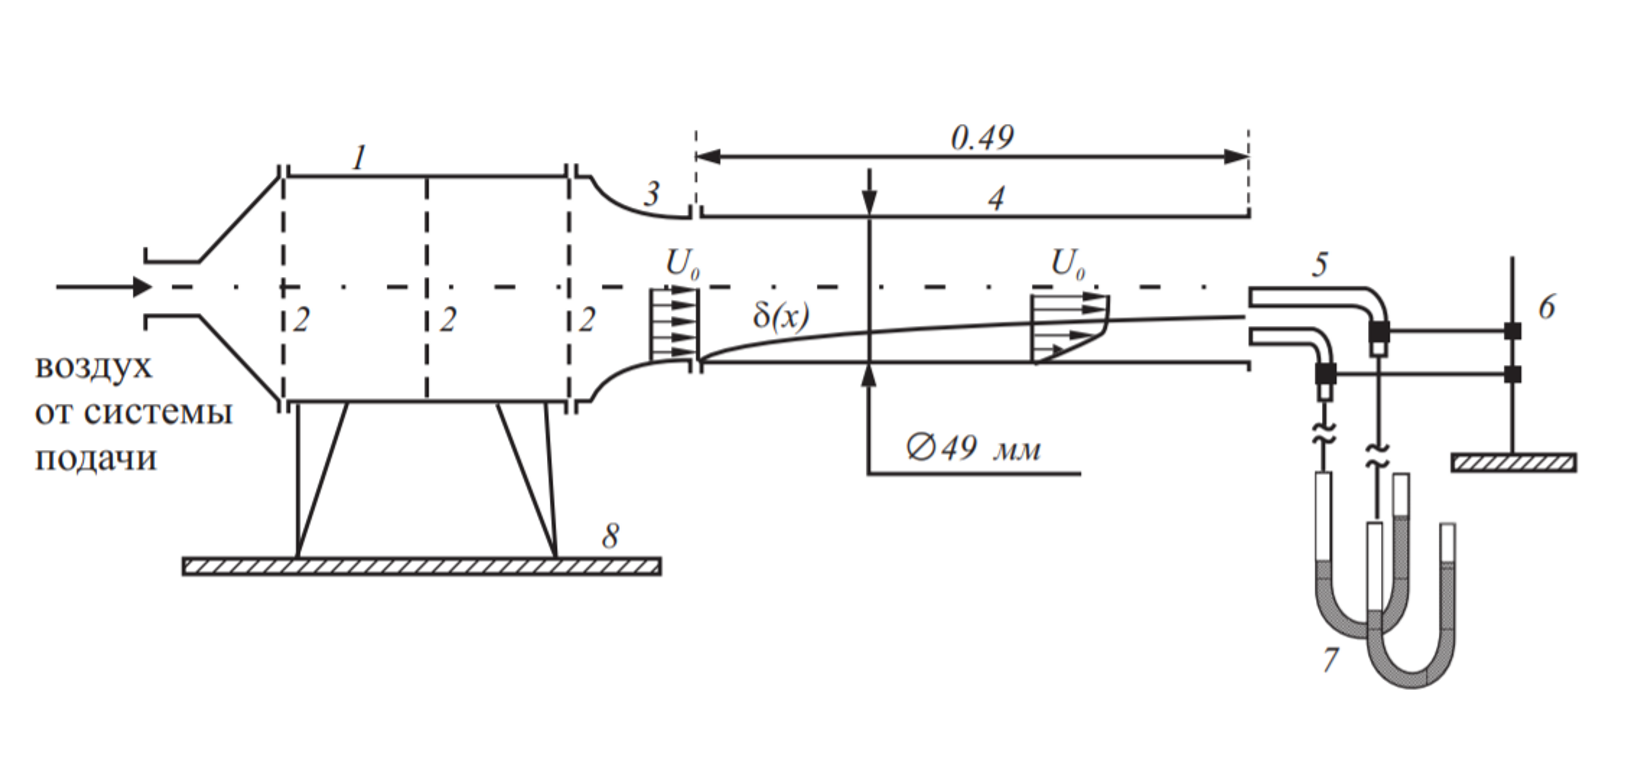
\includegraphics[width=0.9\textwidth]{1.png}
\caption{Cхема установки.}
\end{center}
\end {figure}

На рис. 2 изображены:  1- аэродинамическая дозвуковая труба. 2- система латунных сеток. 3- конфузор. 4- цилиндрический рабочий канал. 5- трубки полного напора. 6-  координатник. 7- манометры. 8- станина.





\section*{Ход работы}

В нашей работе получились следующие значения из пункта "Рассчетные формулы":


$$\rho_\text{атм} = 1.22 \text{ } \frac{\text{кг}}{\text{м}^3}  \text{ -- плотность воздуха}$$

$$ \mu = 1.85 \cdot 10^{-5} \text{ Па} \cdot \text{с} \text{ -- вязкость воздуха} $$


$$u_{\text{я}} = \sqrt{\frac{2\Delta P_{\text{я}}}{\rho_{\text{атм}}}} = k_1 \cdot \sqrt{\Delta P_\text{я}}$$

$$u_{\text{пс}} = \sqrt{\frac{2\Delta P_{\text{пс}}}{\rho_{\text{атм}}}} = k_1 \cdot \sqrt{\Delta P_\text{пс}} $$

$$ k_1 = 1.3 \frac{\text{м/с}}{\sqrt{\text{Па}}} $$ 

где $u_\text{я}$ - скорость в ядре потока, $u_\text{пс}$- скорость в пограничном слое.

\vspace{0.5cm}

Число Рейнольдса:
$$Re_\text{L} = \frac{\rho_\text{атм} L u_\text{я}}{\mu} = \frac{\rho_\text{атм} L}{\mu} k_1 \sqrt{\Delta P_\text{я}} = k_2 \sqrt{\Delta P_\text{я}}$$

$$ k_2 = 4.05 \cdot 10^4 \frac{1}{\sqrt{\text{Па}}} $$


\underline{Примечание:}
Для определения числа Рейнольдса в качестве характерного размера берется длина L опытного участка канала, так как данным размером определяется толщина пограничного слоя в выходном сечении канала, где проводятся все измерения.


\newpage

\subsection*{Определение критического числа Рейнольдса перехода потока от ламинарного к турбулентному}

Изменяя начальную скорость потока во входном сечении аэродинамической трубы путем изменения напряжения, снимем показания манометров в выходном сечении рабочего канала:




\begin{table}[H]
\centering
\begin{tabular}{|c|c|c|c|c|c|}
\hline
$V$, В & $\Delta P_\text{нижняя}$, гПа & $\Delta P_\text{верхняя}$, гПа & $u$/$u_\text{я}$ & $u_\text{я}$ & $Re_L \cdot 10^5$  \\ \hline
80 & 29 & 42 & 0.83 & 8.42 & 2.63 \\ \hline
90 & 40 & 48 & 0.91 & 9.01 & 2.81 \\ \hline
100 & 49 & 56 & 0.94 & 9.73 & 3.03 \\ \hline
110 & 54 & 64 & 0.92 & 10.40 & 3.24 \\ \hline
120 & 55 & 71 & 0.88 & 10.95 & 3.41 \\ \hline
130 & 57 & 80 & 0.84 & 11.63 & 3.62 \\ \hline
140 & 59 & 88 & 0.82 & 12.20 & 3.80 \\ \hline
150 & 62 & 95 & 0.81 & 12.67 & 3.95 \\ \hline
160 & 66 & 104 & 0.80 & 13.26 & 4.13 \\ \hline
180 & 75 & 120 & 0.79 & 14.24 & 4.44 \\ \hline
200 & 84 & 135 & 0.79 & 15.10 & 4.71 \\ \hline
220 & 92 & 149 & 0.785 & 15.87 & 4.95 \\ \hline
240 & 103 & 166 & 0.788 & 16.75 & 5.22 \\ \hline

\end{tabular}
\caption{}
\end{table}

По этим данным построим график $\frac{u}{u_\text{я}} (Re)$
\begin {figure}[H]
\begin{center}
\par
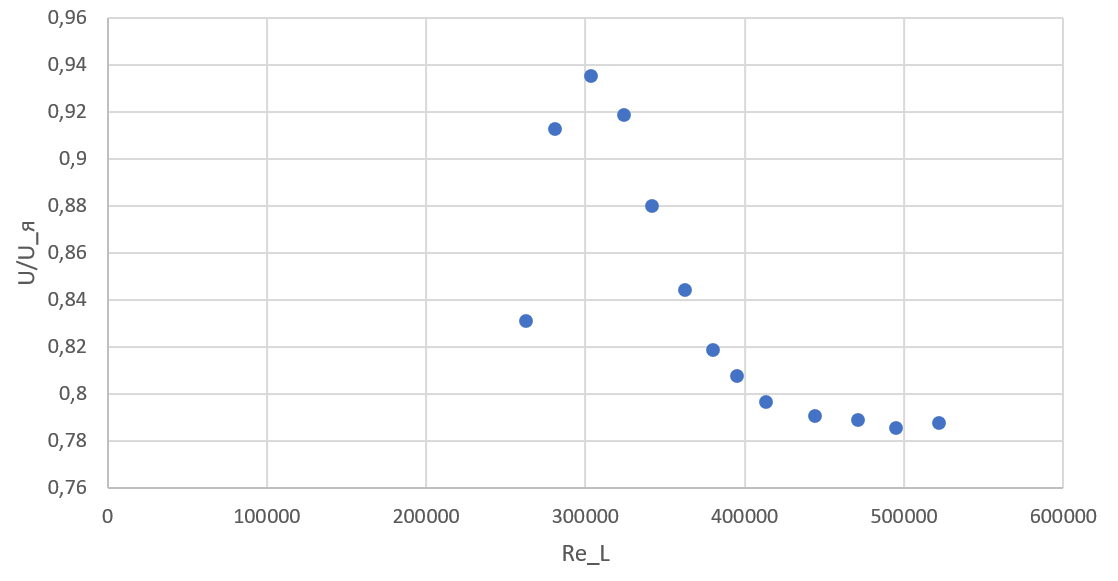
\includegraphics[width=0.9\textwidth]{u-uz.png}
\caption{}
\end{center}
\end {figure}

Из график $Re_\text{кр} = 3.03 \cdot 10^5$- в этой точке достигается максимум экспериментальных значений.


\subsection*{Исследование скорости на срезе рабочего канала при ламинарном и турбулентном пограничном слое}

Для двух разных значений скорости входного потока (соответствующих напряжениям $V = 100$В и $V = 220$В) снимем зависимость давления в пограничном слое от координаты: $V = 100$В (ламинарный пограничный слой):

\begin{table}[H]
\centering
\begin{tabular}{|c|c|c|}
\hline
 $y$, мм & $\Delta P$, Па & $u$/$u_\text{я}$ \\ \hline
0.25 & 2 & 0.038  \\ \hline
0.50 & 3 & 0.057  \\ \hline
0.75 & 8 & 0.151  \\ \hline
1.00 & 12 & 0.226  \\ \hline
1.50 & 24 & 0.453  \\ \hline
2.00 & 35 & 0.660  \\ \hline
2.50 & 44 & 0.830  \\ \hline
3.25 & 52 & 0.981  \\ \hline
4.00 & 53 & 1.000  \\ \hline
5.00 & 54 & 1.019  \\ \hline
5.50 & 54 & 1.019  \\ \hline

\end{tabular}
\caption{Для V = 100В}
\end{table}




\begin{table}[H]
\centering
\begin{tabular}{|c|c|c|}
\hline
 $y$, мм & $\Delta P$, Па & $u$/$u_\text{я}$ \\ \hline
0.25 & 5 & 0.030  \\ \hline
0.50 & 22 & 0.133 \\ \hline
0.75 & 50 & 0.301  \\ \hline
1.00 & 60 & 0.361  \\ \hline
1.50 & 72 & 0.434  \\ \hline
2.00 & 80 & 0.482  \\ \hline
2.50 & 86 & 0.518  \\ \hline
3.25 & 95 & 0.572  \\ \hline
4.00 & 105 & 0.633  \\ \hline
5.00 & 116 & 0.700  \\ \hline
6.00 & 124 & 0.747  \\ \hline
7.00 & 132 & 0.795  \\ \hline

\end{tabular}
\caption{Для V = 220В}
\end{table}

\begin {figure}[H]
\begin{center}
\par
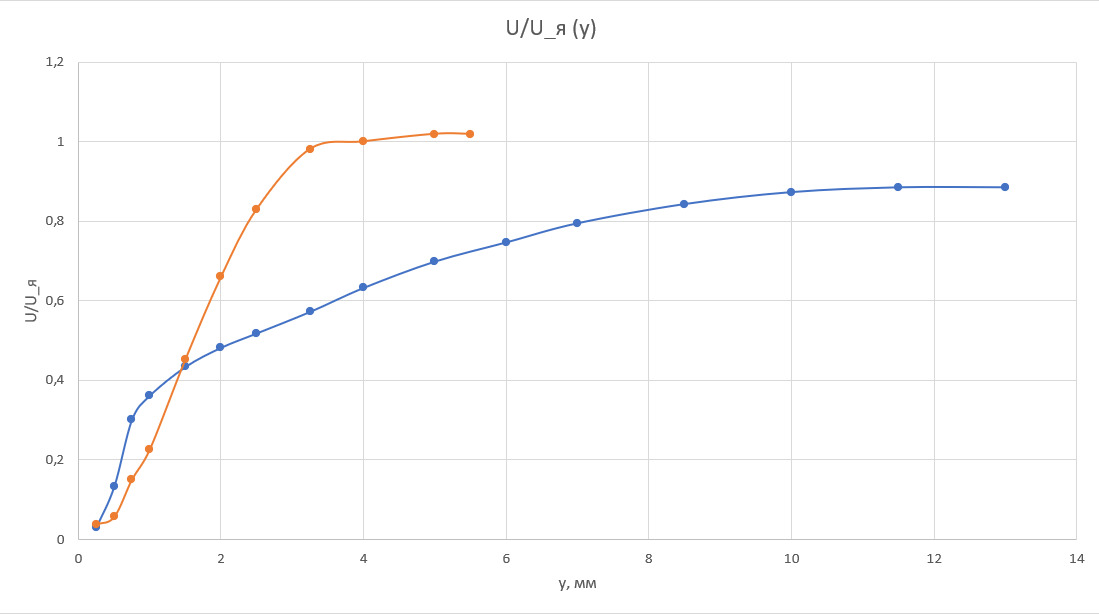
\includegraphics[width=0.9\textwidth]{uuz.png}
\caption{}
\end{center}
\end {figure}


Ламинарное течение: $Re = 2.98 \cdot 10^5 < Re_\text{кр}$
Турбулентное течение: $Re = 4.91 \cdot 10^5 > Re_\text{кр} $

\section*{Вывод:}

В результате данной работы исследовали переход ламинарного течения в пограничном слое несжимаемой жидкости к турбулентному, определили границу перехода между данными режимами, а также вычислили критическое число Рейнольдса:  

$$Re_\text{кр} = 331400$$

Подтверждением справделивости данного значения может являться график на Рис.6 . На нём видно, что при Re < $Re_\text{кр}$ течение в пограничном слое носит ламинарный характер, а при Re > $Re_\text{кр}$ характер течения турбулентный.


Течение в ядре носит турбулентный характер, а пограничный слой имеет область, течение в которой ламинарное, это происходит вследствие \underline{влияния молекулярных сил}. Турбулентность приходит из ядра в пограничный слой в результате возрастания пульсаций, которые с течением времени перестают компенсироваться механизмами сил молекулярной вязкости.

Во всей работе мы пользовались теорией несжимаемой жидкости. Справедливость её применения предтавлена в \textbf{Приложении}.

\newpage
\section*{Приложение}
\section*{Справедливость применения теории несжимаемой жидкости:}

По определению, число Маха (Mach) есть 
$$ M = \frac{v}{a}$$
где $v$- скорость потока, $a$- скорость звука (локальная)

Оно характеризуем меру сжимаемости среды в потоке при заданной скорости.
Из уравнения состояния:
$$\frac{d \rho}{\rho} \sim \frac{dp}{p}$$

Из Бернулли $dp\sim \rho v^2$, таким образом:

$$\frac{d \rho}{\rho} \sim \frac{dp}{p} \sim \frac{\rho v^2}{p}$$

Скорость звука $a \sim \sqrt{p / \rho}$. Относительное изменение плотности в газовом потоке $\sim M^2$:
$$\frac{d \rho}{\rho} \sim \frac{v^2}{a^2} = M^2 \sim 2 \cdot 10^{-4}$$

Это и является подтверждением того, что жидкость в нашей работе можно считать несжимаемой.


\end{document}